%%%%%%%%%%%%%%%%%%%%%%%%%%%%%%%%%%%%%%%%%%%%%%%%%%%%%%%%%%%%%%%%%%%%%%%%%%%%%%%%%%
\begin{frame}[fragile]\frametitle{}
\begin{center}
{\Large Overview of Prompt Engineering}
\end{center}
\end{frame}

%%%%%%%%%%%%%%%%%%%%%%%%%%%%%%%%%%%%%%%%%%%%%%%%%%%%%%%%%%%
\begin{frame}[fragile]\frametitle{New Programming Language?}

\begin{center}

\includegraphics[width=0.8\linewidth,keepaspectratio]{promptengg1}

{\tiny (Ref: Prompt Engineering Sudalai Rajkumar)}

\end{center}				

\end{frame}



%%%%%%%%%%%%%%%%%%%%%%%%%%%%%%%%%%%%%%%%%%%%%%%%%%%%%%%%%%%
\begin{frame}[fragile]\frametitle{What is Prompt Engineering?}

Prompt engineering is a NLP concept that involves discovering inputs that yield desirable or useful results


\begin{center}
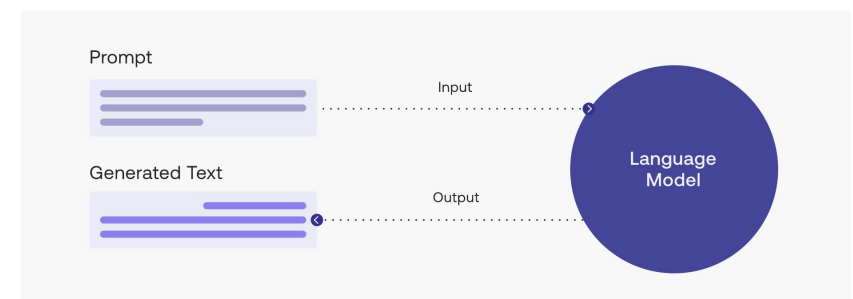
\includegraphics[width=\linewidth,keepaspectratio]{promptengg2}

{\tiny (Ref: Cohere https://docs.cohere.ai/docs/prompt-engineering)}

\end{center}				
			
			

\end{frame}


%%%%%%%%%%%%%%%%%%%%%%%%%%%%%%%%%%%%%%%%%%%%%%%%%%%%%%%%%%%
\begin{frame}[fragile]\frametitle{What is Prompt Engineering?}

How to talk to AI to get it to do what you want


\begin{center}
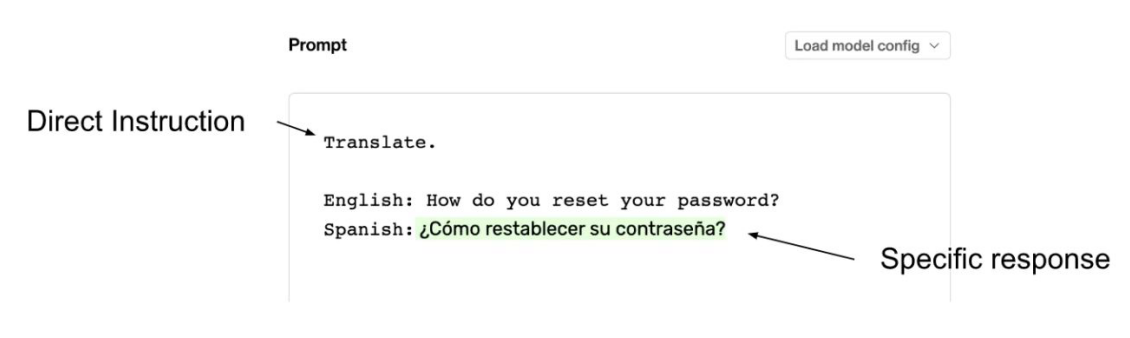
\includegraphics[width=\linewidth,keepaspectratio]{promptengg3}

{\tiny (Ref: Human Loop https://humanloop.com/blog/prompt-engineering-101)}

\end{center}				
			
			

\end{frame}

%%%%%%%%%%%%%%%%%%%%%%%%%%%%%%%%%%%%%%%%%%%%%%%%%%%%%%%%%%%
\begin{frame}[fragile]\frametitle{What is Prompt Engineering?}

But need to tell, for sure, else, nothing


\begin{center}
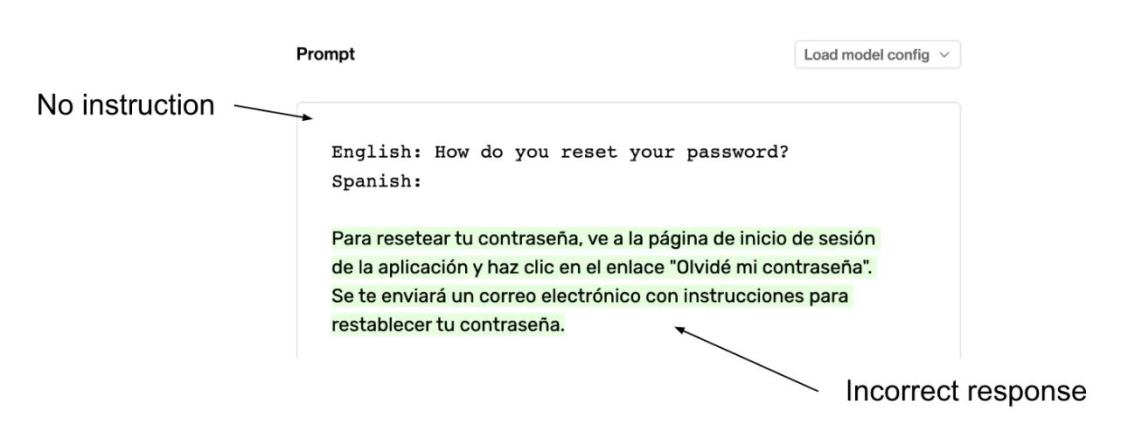
\includegraphics[width=\linewidth,keepaspectratio]{promptengg4}

{\tiny (Ref: Human Loop https://humanloop.com/blog/prompt-engineering-101)}

\end{center}				

\end{frame}


%%%%%%%%%%%%%%%%%%%%%%%%%%%%%%%%%%%%%%%%%%%%%%%%%%%%%%%%%%%
\begin{frame}[fragile]\frametitle{What is Prompt Engineering?}

\begin{itemize}
\item For prompt \lstinline|What is 1,000,000 * 9,000?| GPT-3 (text-davinci-002) (an AI) sometimes answers 9,000,000 (incorrect). This is where prompt engineering comes in.
\item If, instead of asking What is \lstinline|1,000,000 * 9,000?|, we ask \lstinline|What is 1,000,000 * 9,000? Make sure to put the right amount of zeros, even if there are many:|, GPT-3 will answer 9,000,000,000 (correct). 
\item Why is this the case? Why is the additional specification of the number of zeros necessary for the AI to get the right answer? How can we create prompts that yield optimal results on our task? 			
\item That's Prompt Engineering.
\end{itemize}

{\tiny (Ref: https://learnprompting.org/docs/basics/prompting)}
\end{frame}

%%%%%%%%%%%%%%%%%%%%%%%%%%%%%%%%%%%%%%%%%%%%%%%%%%%%%%%%%%%
\begin{frame}[fragile]\frametitle{Elements of Prompt}

A prompt is composed of:

\begin{center}
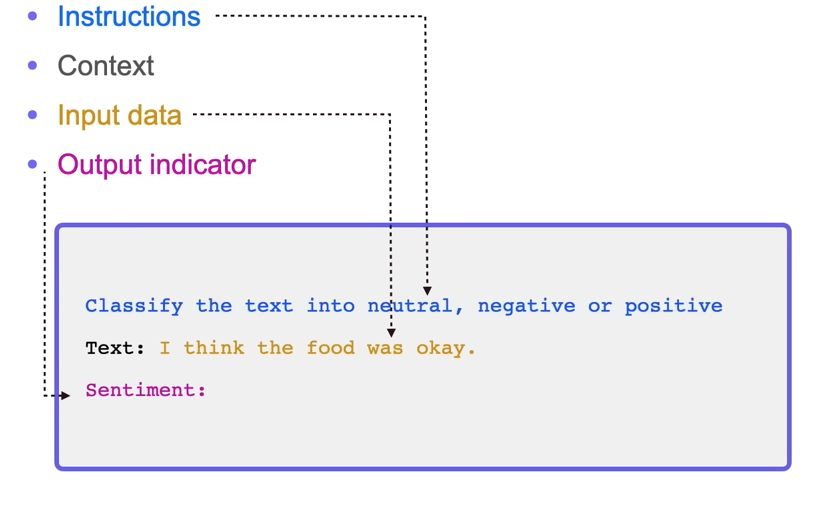
\includegraphics[width=0.8\linewidth,keepaspectratio]{promptengg28}

{\tiny (Ref: Prompt Engineering Overview - Elvis Saravia)}

\end{center}		
		
\end{frame}

%%%%%%%%%%%%%%%%%%%%%%%%%%%%%%%%%%%%%%%%%%%%%%%%%%%%%%%%%%%
\begin{frame}[fragile]\frametitle{Settings of Prompt}

\begin{itemize}
\item 'temperature':  before applying the softmax function, temperature is used scale the logits. With it, creativity or variability is allowed. If you re-run the prompt, with 0, no change, but with 1, lots of variation. Default is 0.7. With a temperature between 0 and 1, we can control the randomness and creativity of the model’s predictions.
\item 'top\_p' or 'nucleus sampling': specifies a sampling threshold during inference time, words passing the threshold are sampled for the output.
\item Like the temperature, the top p parameter controls the randomness and originality of the model.
\item OpenAI documentation recommends using either one parameter or the other and setting the unused parameter to the neutral case, i.e. 1.0.
\end{itemize}
		
\end{frame}


%%%%%%%%%%%%%%%%%%%%%%%%%%%%%%%%%%%%%%%%%%%%%%%%%%%%%%%%%%%
\begin{frame}[fragile]\frametitle{New Roles?}

Coming up with good prompt is a combination of art and science

\begin{center}

\includegraphics[width=0.8\linewidth,keepaspectratio]{promptengg5}

{\tiny (Ref: Prompt Engineering Sudalai Rajkumar)}

\end{center}		
		


\end{frame}

%%%%%%%%%%%%%%%%%%%%%%%%%%%%%%%%%%%%%%%%%%%%%%%%%%%%%%%%%%%

\begin{frame}[fragile]\frametitle{Read on to learn how to engineer good prompts!}

\begin{itemize}
\item Shin, T., Razeghi, Y., Logan IV, R. L., Wallace, E., \& Singh, S. (2020). AutoPrompt: Eliciting Knowledge from Language Models with Automatically Generated Prompts. Proceedings of the 2020 Conference on Empirical Methods in Natural Language Processing (EMNLP). https://doi.org/10.18653/v1/2020.emnlp-main.346 
\item Kojima, T., Gu, S. S., Reid, M., Matsuo, Y., \& Iwasawa, Y. (2022). Large Language Models are Zero-Shot Reasoners. 
\item Liu, P., Yuan, W., Fu, J., Jiang, Z., Hayashi, H., \& Neubig, G. (2022). Pre-train, Prompt, and Predict: A Systematic Survey of Prompting Methods in Natural Language Processing. ACM Computing Surveys. https://doi.org/10.1145/3560815 
\item Brown, T. B., Mann, B., Ryder, N., Subbiah, M., Kaplan, J., Dhariwal, P., Neelakantan, A., Shyam, P., Sastry, G., Askell, A., Agarwal, S., Herbert-Voss, A., Krueger, G., Henighan, T., Child, R., Ramesh, A., Ziegler, D. M., Wu, J., Winter, C., … Amodei, D. (2020). Language Models are Few-Shot Learners. 
\item Zhao, T. Z., Wallace, E., Feng, S., Klein, D., \& Singh, S. (2021). Calibrate Before Use: Improving Few-Shot Performance of Language Models.
\end{itemize}
\end{frame}


%%%%%%%%%%%%%%%%%%%%%%%%%%%%%%%%%%%%%%%%%%%%%%%%%%%%%%%%%%%%%%%%%%%%%%%%%%%%%%%%%%
\begin{frame}[fragile]\frametitle{}
\begin{center}
{\Large Types of Prompts}
\end{center}
\end{frame}


%%%%%%%%%%%%%%%%%%%%%%%%%%%%%%%%%%%%%%%%%%%%%%%%%%%%%%%%%%%
\begin{frame}[fragile]\frametitle{Prompting by Instruction}

\begin{center}
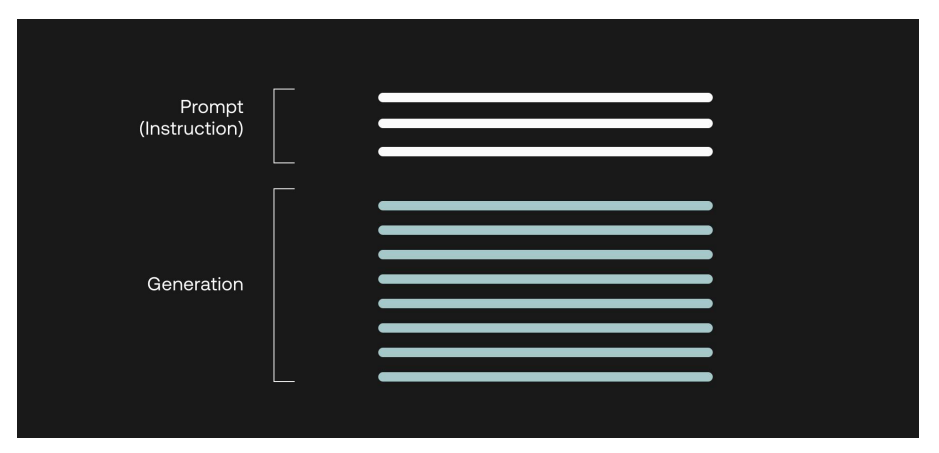
\includegraphics[width=\linewidth,keepaspectratio]{promptengg6}

{\tiny (Ref: Cohere https://txt.cohere.ai/generative-ai-part-1/)}

\end{center}		
		


\end{frame}

%%%%%%%%%%%%%%%%%%%%%%%%%%%%%%%%%%%%%%%%%%%%%%%%%%%%%%%%%%%
\begin{frame}[fragile]\frametitle{Example: Prompting by Instruction}

\begin{center}
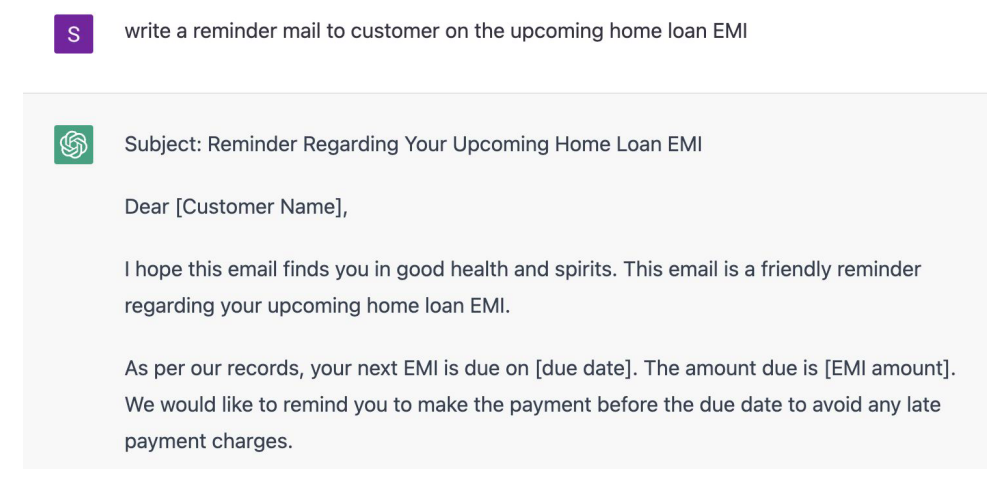
\includegraphics[width=\linewidth,keepaspectratio]{promptengg7}

{\tiny (Ref: Cohere https://txt.cohere.ai/generative-ai-part-1/)}

\end{center}		
		


\end{frame}

%%%%%%%%%%%%%%%%%%%%%%%%%%%%%%%%%%%%%%%%%%%%%%%%%%%%%%%%%%%
\begin{frame}[fragile]\frametitle{Prompting by Examples}

\begin{center}
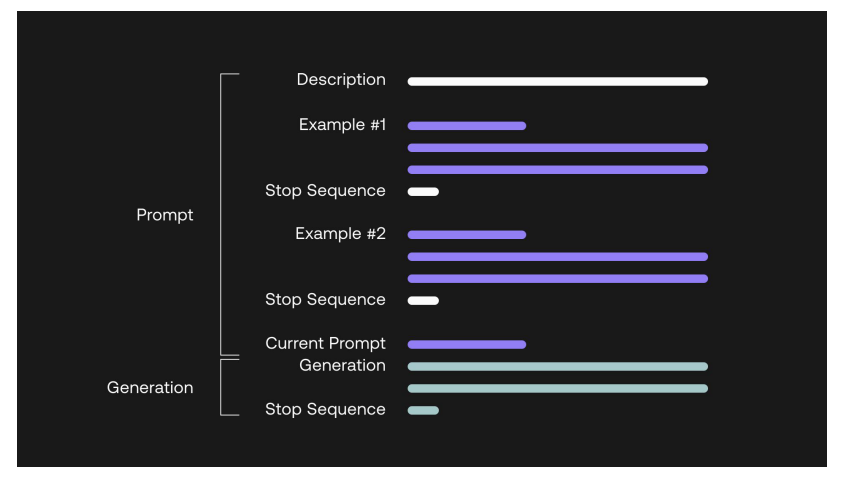
\includegraphics[width=\linewidth,keepaspectratio]{promptengg8}

{\tiny (Ref: Cohere https://txt.cohere.ai/generative-ai-part-1/)}

\end{center}		
		


\end{frame}

%%%%%%%%%%%%%%%%%%%%%%%%%%%%%%%%%%%%%%%%%%%%%%%%%%%%%%%%%%%
\begin{frame}[fragile]\frametitle{Example: Prompting by Examples}

\begin{center}
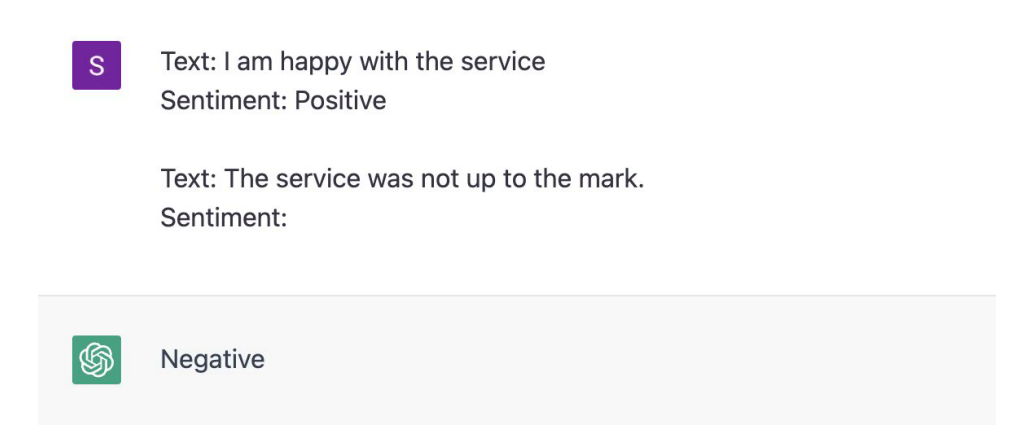
\includegraphics[width=\linewidth,keepaspectratio]{promptengg9}

{\tiny (Ref: Cohere https://txt.cohere.ai/generative-ai-part-1/)}

\end{center}		
		
\end{frame}

%%%%%%%%%%%%%%%%%%%%%%%%%%%%%%%%%%%%%%%%%%%%%%%%%%%%%%%%%%%%%%%%%%%%%%%%%%%%%%%%%%
\begin{frame}[fragile]\frametitle{}
\begin{center}
{\Large Applications of Prompts}
\end{center}
\end{frame}

%%%%%%%%%%%%%%%%%%%%%%%%%%%%%%%%%%%%%%%%%%%%%%%%%%%%%%%%%%%
\begin{frame}[fragile]\frametitle{Text Generation}

\begin{center}
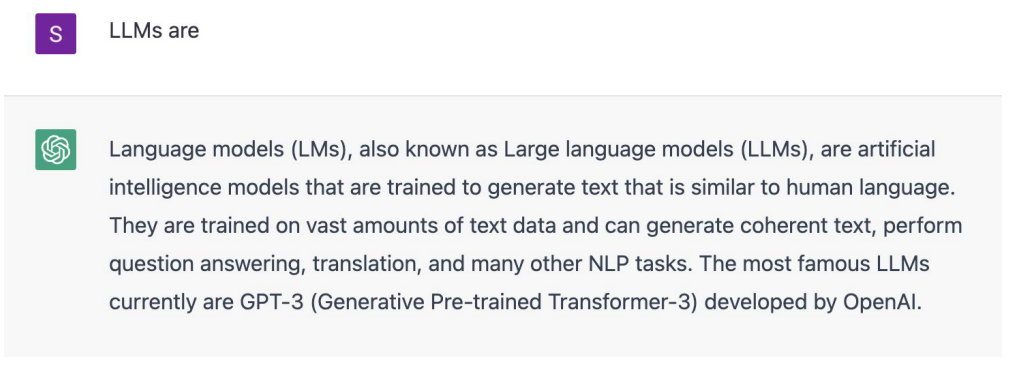
\includegraphics[width=\linewidth,keepaspectratio]{promptengg10}

{\tiny (Ref: Prompt Engineering Sudalai Rajkumar)}

\end{center}		
		


\end{frame}

%%%%%%%%%%%%%%%%%%%%%%%%%%%%%%%%%%%%%%%%%%%%%%%%%%%%%%%%%%%
\begin{frame}[fragile]\frametitle{Text Classification}

\begin{center}
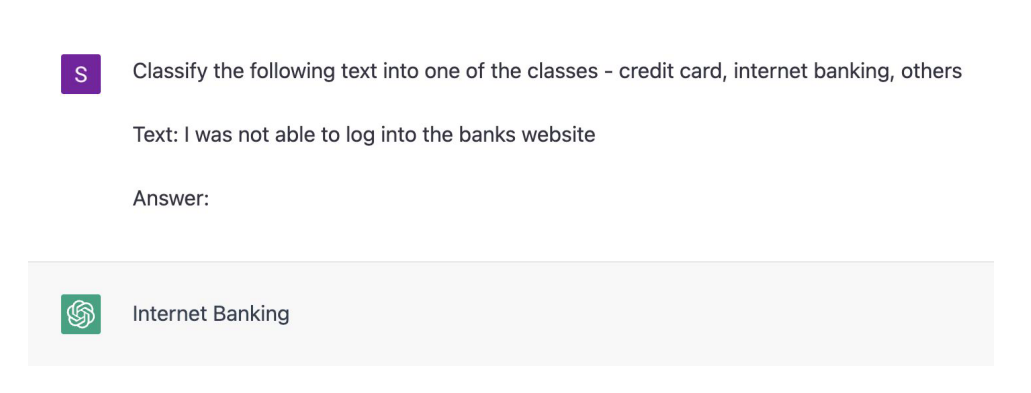
\includegraphics[width=\linewidth,keepaspectratio]{promptengg11}

{\tiny (Ref: Prompt Engineering Sudalai Rajkumar)}

\end{center}		
		


\end{frame}

%%%%%%%%%%%%%%%%%%%%%%%%%%%%%%%%%%%%%%%%%%%%%%%%%%%%%%%%%%%
\begin{frame}[fragile]\frametitle{Text Translation}

\begin{center}

\includegraphics[width=\linewidth,keepaspectratio]{promptengg12}

{\tiny (Ref: Prompt Engineering Sudalai Rajkumar)}

\end{center}		
		


\end{frame}

%%%%%%%%%%%%%%%%%%%%%%%%%%%%%%%%%%%%%%%%%%%%%%%%%%%%%%%%%%%
\begin{frame}[fragile]\frametitle{Text Comprehension}

\begin{center}
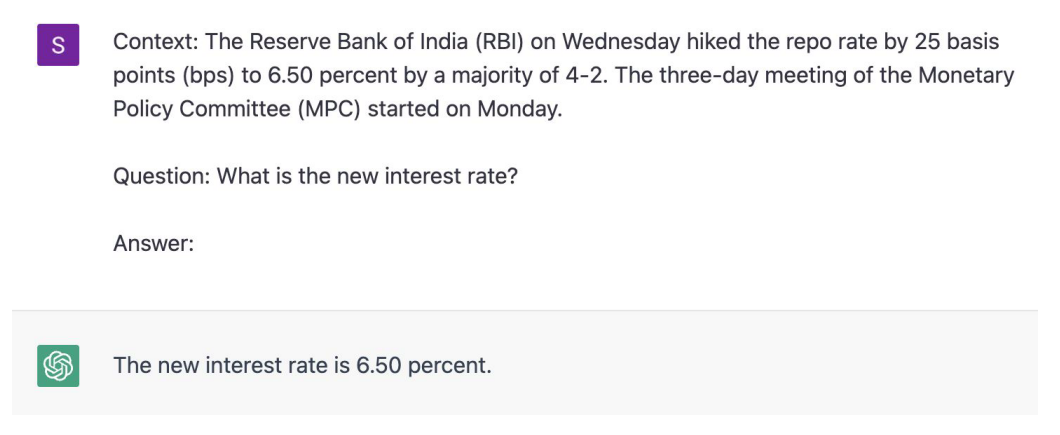
\includegraphics[width=\linewidth,keepaspectratio]{promptengg13}

{\tiny (Ref: Prompt Engineering Sudalai Rajkumar)}

\end{center}		
		


\end{frame}

%%%%%%%%%%%%%%%%%%%%%%%%%%%%%%%%%%%%%%%%%%%%%%%%%%%%%%%%%%%
\begin{frame}[fragile]\frametitle{Text Summarization}

\begin{center}
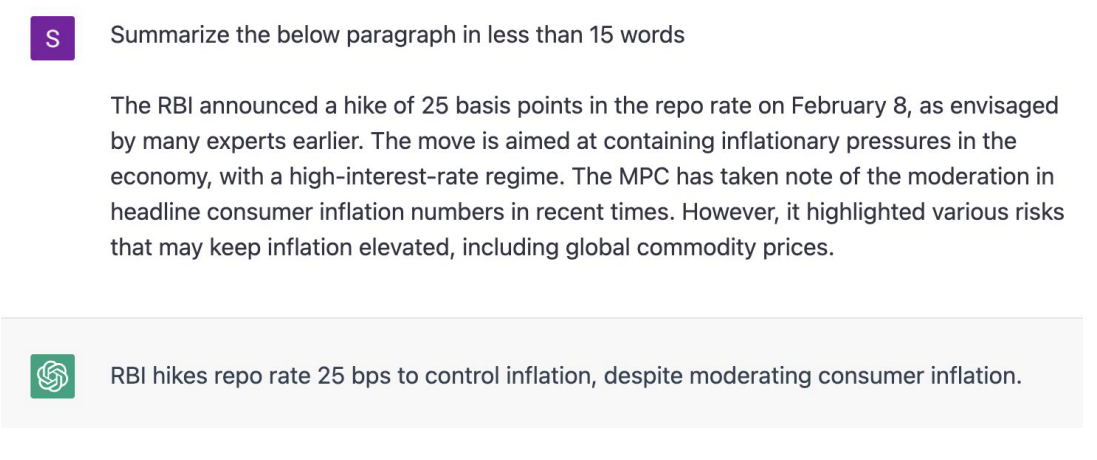
\includegraphics[width=\linewidth,keepaspectratio]{promptengg14}

{\tiny (Ref: Prompt Engineering Sudalai Rajkumar)}

\end{center}		
		


\end{frame}

%%%%%%%%%%%%%%%%%%%%%%%%%%%%%%%%%%%%%%%%%%%%%%%%%%%%%%%%%%%
\begin{frame}[fragile]\frametitle{Image Generation}

\begin{center}
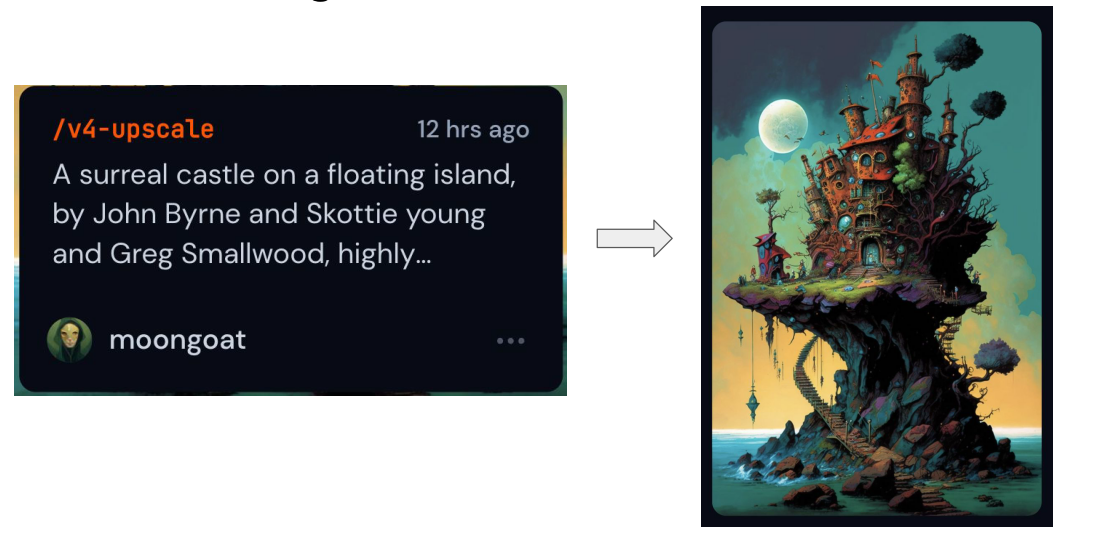
\includegraphics[width=\linewidth,keepaspectratio]{promptengg15}

{\tiny (Ref: Prompt Engineering Sudalai Rajkumar)}

\end{center}		
		
		
Models / Tools: Dall-E , Midjourney, Stable Diffusion



\end{frame}


%%%%%%%%%%%%%%%%%%%%%%%%%%%%%%%%%%%%%%%%%%%%%%%%%%%%%%%%%%%%%%%%%%%%%%%%%%%%%%%%%%
\begin{frame}[fragile]\frametitle{}
\begin{center}
{\Large Design of Prompts}
\end{center}
\end{frame}

%%%%%%%%%%%%%%%%%%%%%%%%%%%%%%%%%%%%%%%%%%%%%%%%%%%%%%%%%%%
\begin{frame}[fragile]\frametitle{Length Control}

Specify a desired word count or character count as part of the prompt

\begin{center}
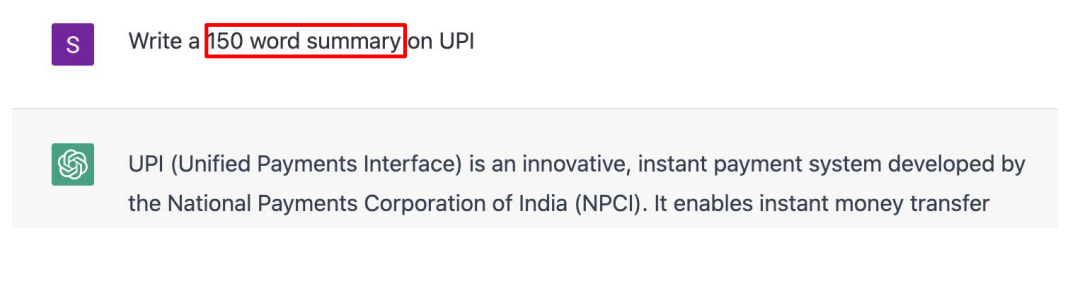
\includegraphics[width=\linewidth,keepaspectratio]{promptengg16}

{\tiny (Ref: Prompt Engineering Sudalai Rajkumar)}

\end{center}		
		
		


\end{frame}

%%%%%%%%%%%%%%%%%%%%%%%%%%%%%%%%%%%%%%%%%%%%%%%%%%%%%%%%%%%
\begin{frame}[fragile]\frametitle{Tone Control}

Specify specific words or phrases that indicate the desired tone

\begin{center}
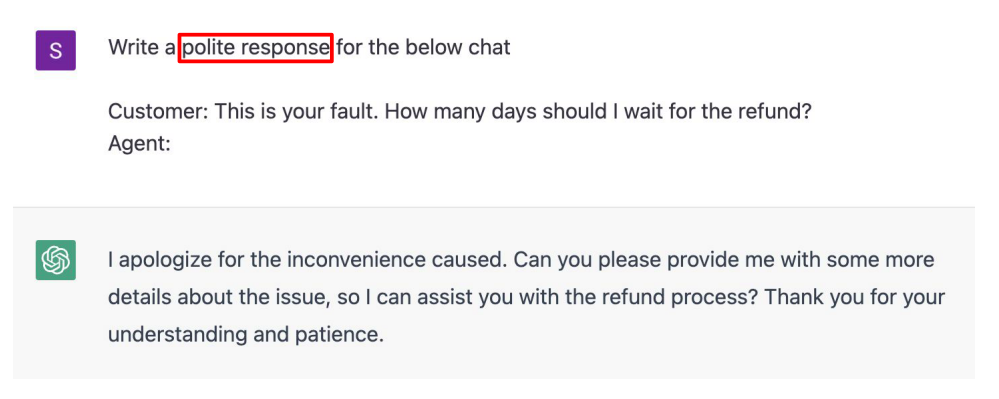
\includegraphics[width=\linewidth,keepaspectratio]{promptengg17}

{\tiny (Ref: Prompt Engineering Sudalai Rajkumar)}

\end{center}		
		
		


\end{frame}

%%%%%%%%%%%%%%%%%%%%%%%%%%%%%%%%%%%%%%%%%%%%%%%%%%%%%%%%%%%
\begin{frame}[fragile]\frametitle{Style Control}

Specify the desired writing style.

\begin{center}
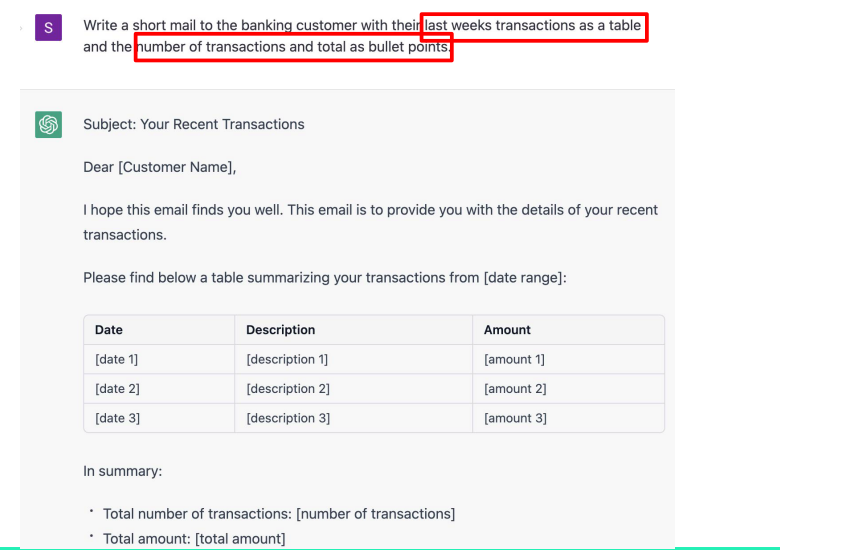
\includegraphics[width=\linewidth,keepaspectratio]{promptengg18}

{\tiny (Ref: Prompt Engineering Sudalai Rajkumar)}

\end{center}		
		
		


\end{frame}

%%%%%%%%%%%%%%%%%%%%%%%%%%%%%%%%%%%%%%%%%%%%%%%%%%%%%%%%%%%
\begin{frame}[fragile]\frametitle{Audience Control}

Specify the desired audience.

\begin{center}
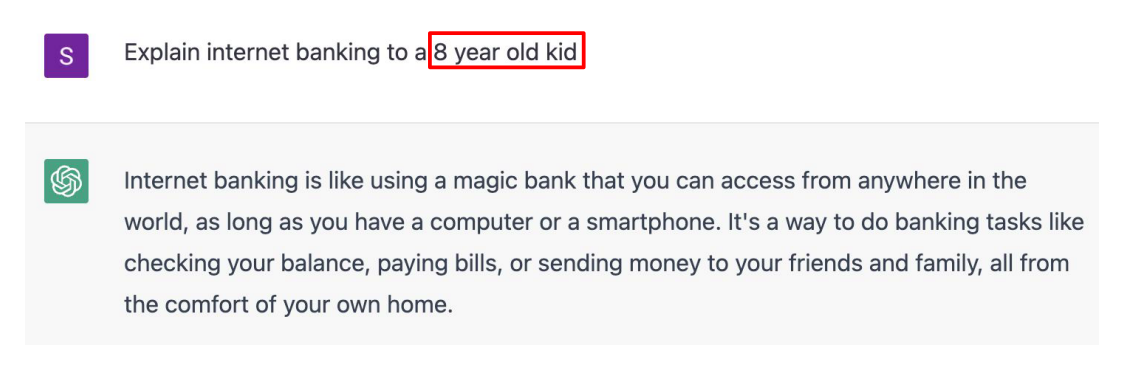
\includegraphics[width=\linewidth,keepaspectratio]{promptengg19}

{\tiny (Ref: Prompt Engineering Sudalai Rajkumar)}

\end{center}		


\end{frame}

%%%%%%%%%%%%%%%%%%%%%%%%%%%%%%%%%%%%%%%%%%%%%%%%%%%%%%%%%%%
\begin{frame}[fragile]\frametitle{Context Control}

Specify the information about the context.

\begin{center}
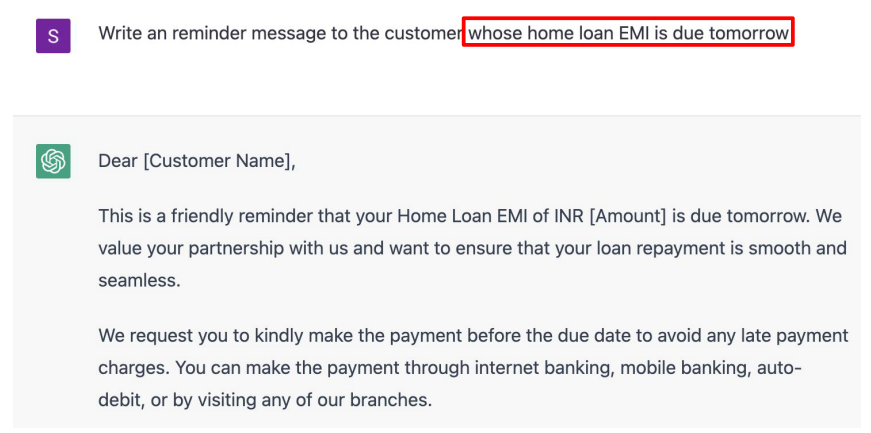
\includegraphics[width=\linewidth,keepaspectratio]{promptengg20}

{\tiny (Ref: Prompt Engineering Sudalai Rajkumar)}

\end{center}		
		
		


\end{frame}

%%%%%%%%%%%%%%%%%%%%%%%%%%%%%%%%%%%%%%%%%%%%%%%%%%%%%%%%%%%
\begin{frame}[fragile]\frametitle{ Keyword Based Guiding}

To guide the model towards specific outputs, the prompt can include 
keywords that are relevant to the desired output

\begin{center}
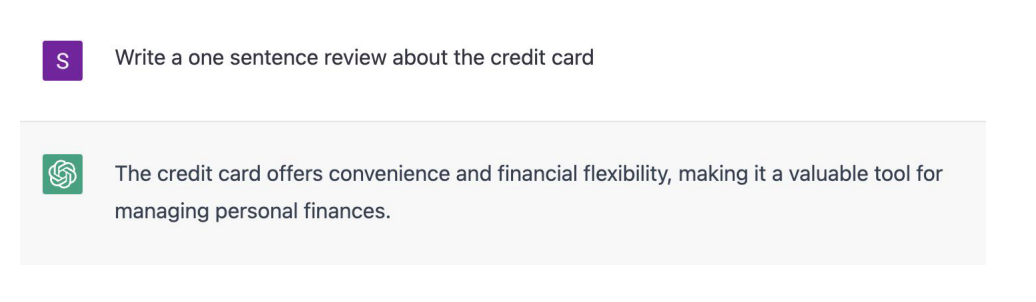
\includegraphics[width=\linewidth,keepaspectratio]{promptengg21}

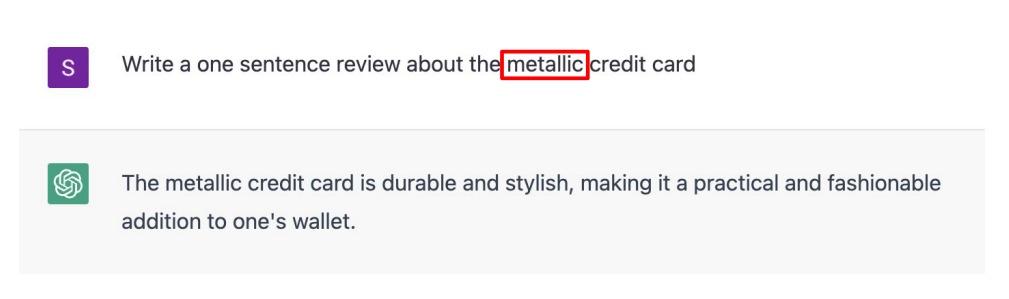
\includegraphics[width=\linewidth,keepaspectratio]{promptengg22}

{\tiny (Ref: Prompt Engineering Sudalai Rajkumar)}

\end{center}		
		
		
		


\end{frame}

%%%%%%%%%%%%%%%%%%%%%%%%%%%%%%%%%%%%%%%%%%%%%%%%%%%%%%%%%%%
\begin{frame}[fragile]\frametitle{ Scenario Based Guiding}

The prompt can describe a specific scenario to guide the model towards 
generating text that fits that scenario.

\begin{center}
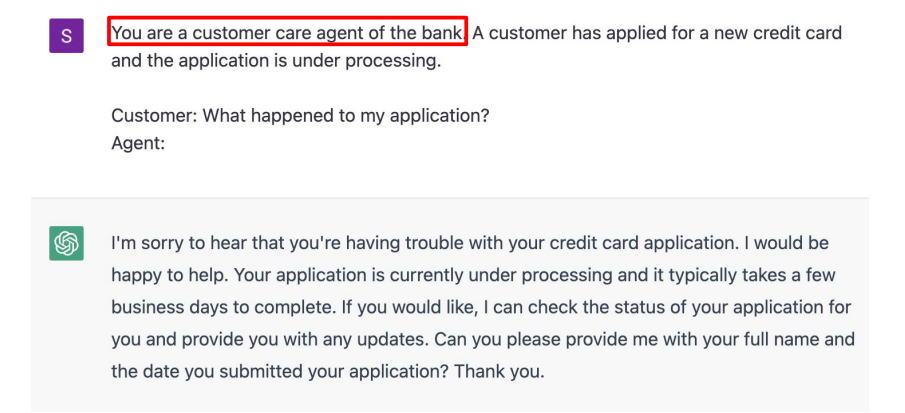
\includegraphics[width=\linewidth,keepaspectratio]{promptengg23}

{\tiny (Ref: Prompt Engineering Sudalai Rajkumar)}

\end{center}		
		
		
		


\end{frame}

%%%%%%%%%%%%%%%%%%%%%%%%%%%%%%%%%%%%%%%%%%%%%%%%%%%%%%%%%%%
\begin{frame}[fragile]\frametitle{Chain of Thoughts}

Provides a “chain of thought” process that 
showcases how the correct answer to a question should be reached

\begin{center}
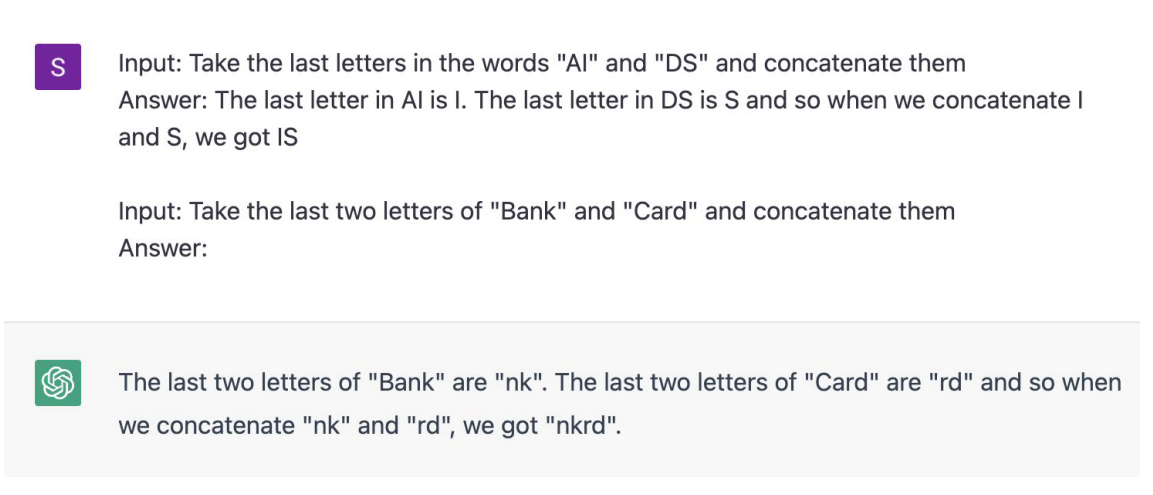
\includegraphics[width=\linewidth,keepaspectratio]{promptengg24}

{\tiny (Ref: Prompt Engineering Sudalai Rajkumar)}

\end{center}		

\end{frame}

%%%%%%%%%%%%%%%%%%%%%%%%%%%%%%%%%%%%%%%%%%%%%%%%%%%%%%%%%%%
\begin{frame}[fragile]\frametitle{Chain of Thoughts (CoT)}

Encourages the LLM to explain its reasoning. 

\begin{center}
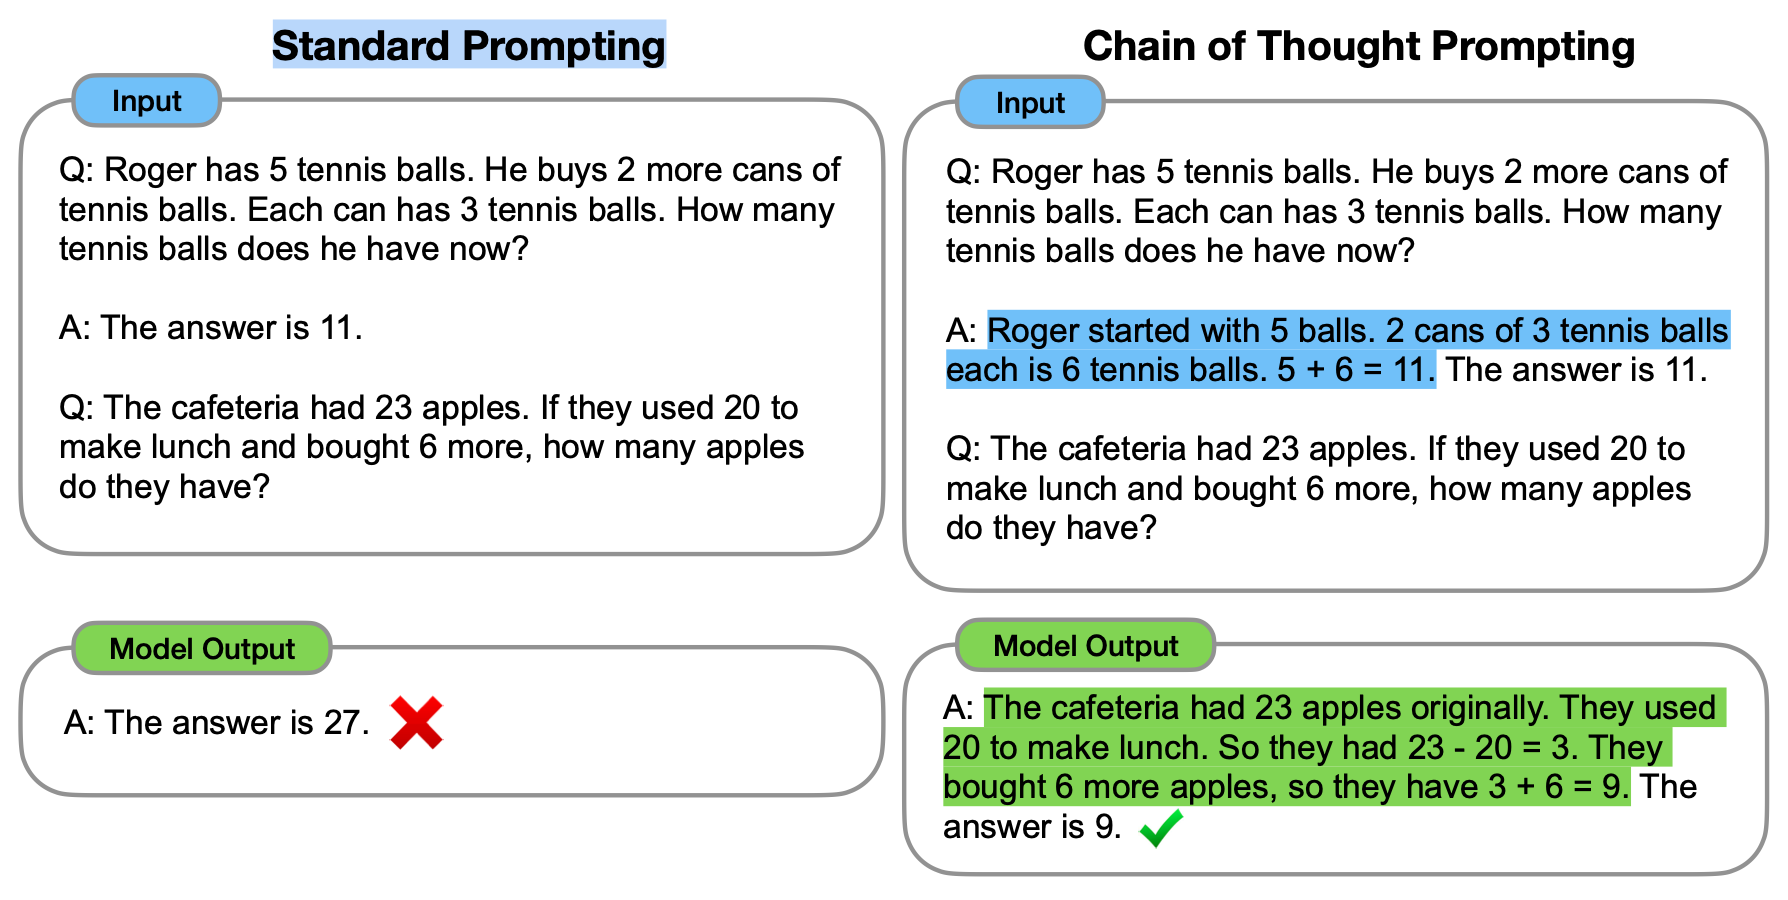
\includegraphics[width=0.8\linewidth,keepaspectratio]{promptengg25}

{\tiny (Ref: https://learnprompting.org/docs/intermediate/chain\_of\_thought)}

\end{center}		

The main idea of CoT is that by showing the LLM some few shot exemplars where the reasoning process is explained in the exemplars, the LLM will also show the reasoning process when answering the prompt. This explanation of reasoning often leads to more accurate results.

\end{frame}

%%%%%%%%%%%%%%%%%%%%%%%%%%%%%%%%%%%%%%%%%%%%%%%%%%%%%%%%%%%
\begin{frame}[fragile]\frametitle{Zero Shot Chain of Thought}

An incredibly simple zero shot prompt. They find that by appending the words "Let's think step by step." to the end of a question, LLMs are able to generate a chain of thought that answers the question. From this chain of thought, they are able to extract more accurate answers.

\begin{center}
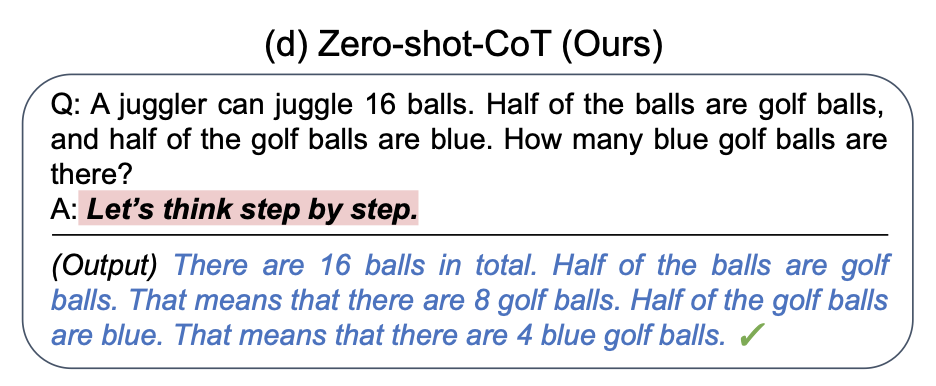
\includegraphics[width=0.8\linewidth,keepaspectratio]{promptengg26}

{\tiny (Ref: https://learnprompting.org/docs/intermediate/zero\_shot\_cot)}

\end{center}		

\end{frame}

%%%%%%%%%%%%%%%%%%%%%%%%%%%%%%%%%%%%%%%%%%%%%%%%%%%%%%%%%%%
\begin{frame}[fragile]\frametitle{Self-Consistency}

Generates multiple chains of thought instead of just one, then takes the majority answer as the final answer.

\begin{center}
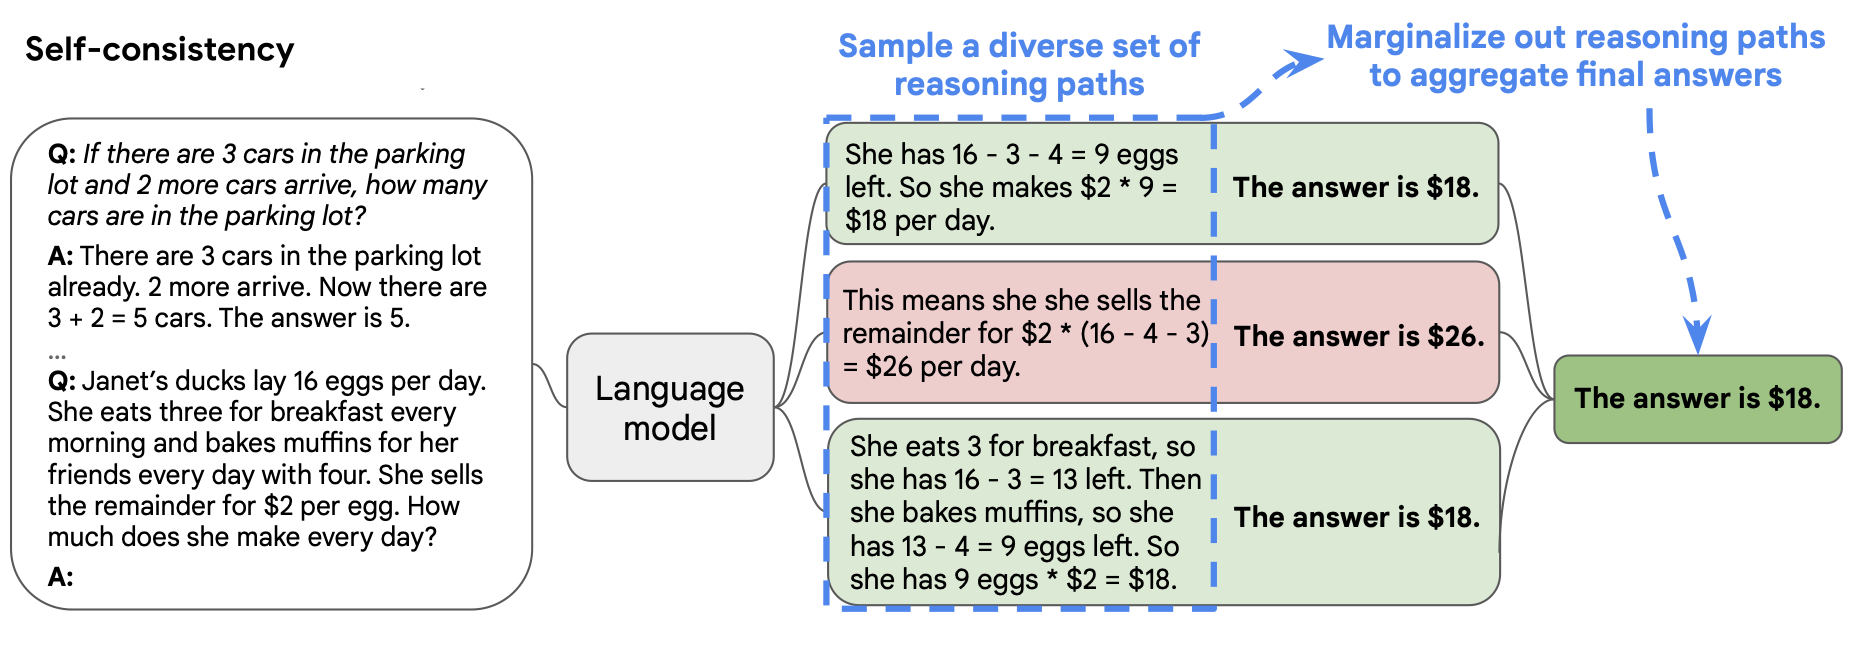
\includegraphics[width=\linewidth,keepaspectratio]{promptengg27}

{\tiny (Ref: https://learnprompting.org/docs/intermediate/self\_consistency)}

\end{center}		

The prompt on the left is written using the Few-Shot-CoT paradigm. Using this one prompt, multiple chains of thought are generated independently. Answers are extracted from each and the final answer is computed by "marginalizing out reasoning paths". In practice, this just means taking the majority answer.

\end{frame}

%%%%%%%%%%%%%%%%%%%%%%%%%%%%%%%%%%%%%%%%%%%%%%%%%%%%%%%%%%%
\begin{frame}[fragile]\frametitle{ Avoiding Unwanted Outputs}


\begin{itemize}
\item  Blacklisting words: ``Write a summary about banks but avoid using the word loans''
\item Topic Constraints: ``Write a review on iphone without covering the price aspect''
\item Output type constraints: ``Write a poem about nature but avoid using rhyming words''
\end{itemize}	 

		
		
{\tiny (Ref: Prompt Engineering Sudalai Rajkumar)}


\end{frame}



%%%%%%%%%%%%%%%%%%%%%%%%%%%%%%%%%%%%%%%%%%%%%%%%%%%%%%%%%%%%%%%%%%%%%%%%%%%%%%%%%%
\begin{frame}[fragile]\frametitle{}
\begin{center}
{\Large Conclusions}
\end{center}
\end{frame}

%%%%%%%%%%%%%%%%%%%%%%%%%%%%%%%%%%%%%%%%%%%%%%%%%%%%%%%%%%%
\begin{frame}[fragile]\frametitle{Limitations}


\begin{itemize}
\item  Size of the language models: GPT index - https://github.com/jerryjliu/gpt\_index
\item Memory \& sequence of calls: LangChain - https://github.com/hwchase17/langchain
\item Correctness of the output
\end{itemize}	 

		
		
{\tiny (Ref: Prompt Engineering Sudalai Rajkumar)}


\end{frame}

%%%%%%%%%%%%%%%%%%%%%%%%%%%%%%%%%%%%%%%%%%%%%%%%%%%%%%%%%%%
\begin{frame}[fragile]\frametitle{My Sketchnote}

\begin{center}
\includegraphics[width=0.45\linewidth,keepaspectratio]{PromptEng_Sketchnote_Medium}

{\tiny (Ref: https://medium.com/technology-hits/prompting-is-all-you-need-5dddb82bd022)}
\end{center}		


			

\end{frame}
